{\sffamily\small\bfseries\color{black}A SHORT MANUAL FOR GENERAL ENGINEERS | 10 OCTOBER 2026}\par\vspace{4mm}
{\sffamily\bfseries\color{black}\fontsize{27}{31}\selectfont A factory alarm, explained\par}
\vspace{3mm}
{\sffamily\large From the animated line to an operator's next decision\par}
\vspace{5mm}
Imagine arriving at a line you have never worked on. Material enters at the top, screws turn, and parcels move along the conveyor. Then a component flashes, a technician walks across the scene, and an AI investigation appears. What actually happened?

This guide follows that story without assuming extrusion or AI experience: meet the machine, follow an alarm, and learn what inspection, repair and restart mean. Then meet the agent backstage: how it gets advice, uses evidence and earns permission to act.

\begin{center}
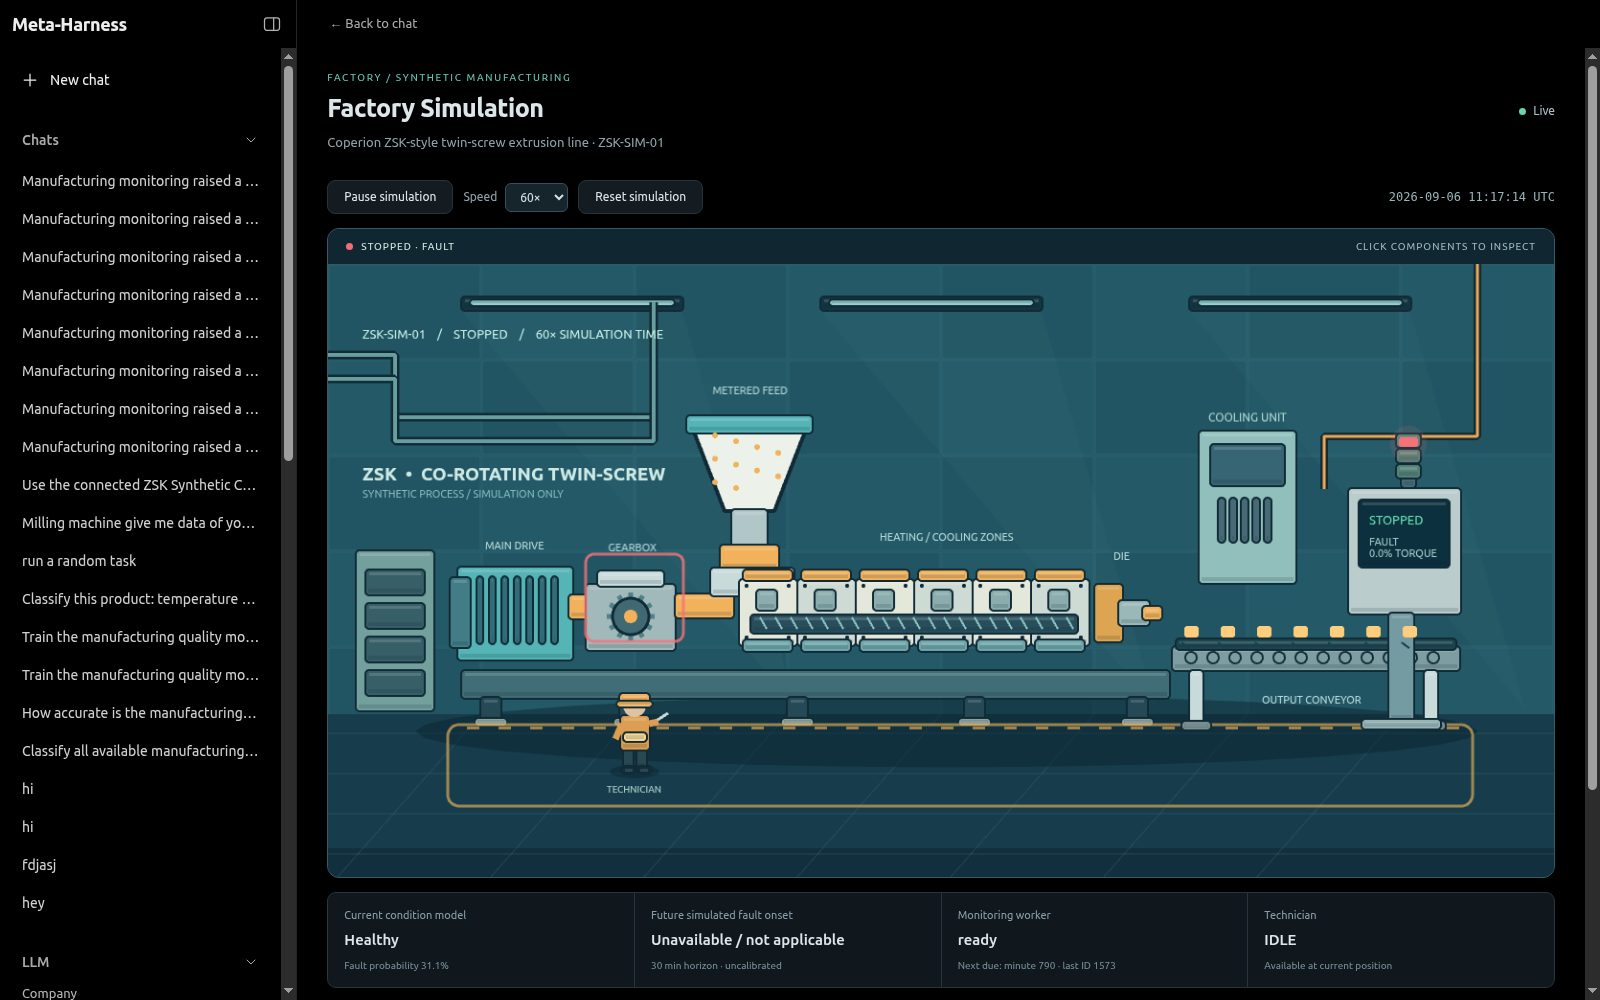
\includegraphics[width=.95\linewidth,trim=327bp 122bp 46bp 228bp,clip]{guide/figures/game-scene.png}
\captionof{figure}{The actual game in a saved browser verification capture: STOPPED / FAULT. The displayed machine is synthetic; no physical line is connected.}
\end{center}

\takeaway{The game displays a synthetic machine. The backend owns its condition, sensors and actions; the AI investigates its records. No physical manufacturing line is connected.}

\subsection*{Follow the story}
\begin{tabularx}{\linewidth}{@{}rXrX@{}}\toprule
2 & Meet the line & 10 & Connect the agent to the LLM\\
3 & Read the signals & 11 & Follow the agent's loop\\
4 & Understand the two models & 12 & Tools and security\\
5 & Watch an investigation & 13 & Consult documents with RAG\\
6 & Understand the animation & 14 & Memory and context\\
7 & Follow a recorded alarm & 15 & Validate and recover\\
8 & Inspect, repair, restart & 16 & Find help and sources\\
9 & Try different problems & & \\\bottomrule
\end{tabularx}

The ZSK-style extruder and its fault effects are illustrative, not a manufacturer maintenance procedure.
